\documentclass{article}
\author{Jim Lam}
\usepackage{hyperref}
\usepackage{amsmath}
\usepackage{amssymb}
\usepackage{tikz}
\usetikzlibrary{automata, positioning, arrows}
\tikzset{
->, % makes the edges directed
node distance=3cm, % specifies the minimum distance between two nodes. Change if necessary.
every state/.style={thick, fill=gray!10}, % sets the properties for each ’state’ node
initial text=$ $, % sets the text that appears on the start arrow
}
\def\firstellip{(1.6, 0) ellipse [x radius=3cm, y radius=1.5cm, rotate=50]}
\def\secondellip{(0.3, 1cm) ellipse [x radius=3cm, y radius=1.5cm,
rotate=50]} \def\thirdellip{(-1.6, 0) ellipse [x radius=3cm, y radius=1.5cm,
rotate=-50]} \def\fourthellip{(-0.3, 1cm) ellipse [x radius=3cm, y
radius=1.5cm, rotate=-50]} \def\bounding{(-5,-3) rectangle (5,4)}
\def\exp{
    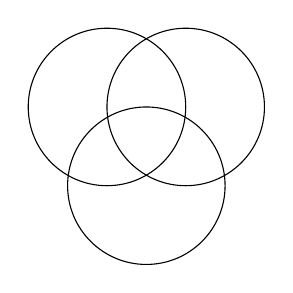
\begin{tikzpicture}
        %% You can adjust the opacity here. For venn diagrams it is convenient to have a low opacity so that you can see intersections
        \begin{scope} [fill opacity = .0]
            %% The draw command knows a lot of shapes. To make a rectangle you just need to specify two diagonal corners. Make sure you always have a semicolon at the end of your draw commands, otherwise latex flips out.
            %% Similarly, you can make a circle by specifying the center and then the radius. You can also add a fill color, but if you're printing in black and white you'll probably want to remove that line.
            \draw[fill=green, draw = black] (-0.5,1) circle (1);
            \draw[fill=blue, draw = black] (0.5,1) circle (1);
            \draw[fill=red, draw = black] (0,0) circle (1);
            %% We can use the node command to label points. If you put your cursor on "LARGE" or "textbf" a box will drop down with size and text style options.
            \node at (-0.9,1.4) {$\mathbf{A}$};
            \node at (0.9,1.4) {$\mathbf{B}$};
            \node at (0, -0.4) {$\mathbf{C}$};
        \end{scope}
        %% And now you have a venn diagram. Yay!
        %\draw[help lines](-5,5) grid (5,-6);    This line can draw the grid lines to help guide you. I use these when I'm writing the code and then delete this line when I publish the pdf.
    \end{tikzpicture}
}
\begin{document}
\title{Notes for COM1026 in semester test 1, condensed from lecture slides}
\maketitle
\tableofcontents
\section{Set Theory}

\subsection{Introduction}
Quick recap on Naive set theory, meaning:

1. Introducing the basic concept of sets;

2. Introduce notation;

3. Illustrate Union, Intersection, and Set Difference operations;

4. Venn diagrams as proof;

5. Power sets;

6. How to proof with more rigor.

\subsection{Set Definition}

Question: Why are sets relevant to computing?

We have to represent data to compute it.
To group data, we put it into sets.

Some sets that I have seen before:
\begin{align*}
    \text{The set of natural numbers: } \mathbb{N} & = \{1, 2, 3, ...\}                    \\
    \text{The set of integers: } \mathbb{Z}        & = \{..., -3, -2, -1, 0, 1, 2, 3,...\}
\end{align*}
Question: What are sets?

% generate a heavily stylised latex quote of the definition of a set below.

A set is a collection of objects, called elements of the set. The elements of a set can be anything, but they must be distinct.

\subsection{Notation}
Sets are denoted with capital letters, e.g. A, B, C. The elements of a set are listed inside curly brackets:
\begin{align*}
    A & = \{1, 2, 3\}                \\
    B & = \{a, b, c, d, e, f, g, h\}
\end{align*}

\subsubsection{Cardinality}

The cardinality of a set is the number of elements in the set. The cardinality of a set is denoted with vertical bars, with the hash, or alternatively, the function $card$:
\begin{align*}
    \text{Card}(A)  & = |A| = 3 \\
    \#\{1,2,3,4,5\} & = 5       \\
    \#A             & = 3       \\  % hash also works.
    \#\mathbb{N}    & = \infty
\end{align*}
\subsubsection{Abstraction axiom}
GIven a property $P(x)$, we can define a set $A$ as:
\begin{align*}
    A & = \{x | P(x)\}
\end{align*}
In other words, whatever property P, there exists a set A containing the objects that satisfy P and only these objects.

\subsubsection{Set builder notation}
Other than enumerating the elements of a set, there are other ways to describe a set. Verbal descriptions and adding an inclusion rule to the set builder notation are two more examples:
\begin{align*}
    C & = \{x | x \in \mathbb{N}, 0 \leq x \leq 5\}                    \\
      & = \{x |\text{$x$ is in the appropriate set}, 0 \leq x \leq 5\}
\end{align*}

\subsubsection{Empty set}
The empty set is a set with no elements. It is denoted $\emptyset$ or $\{\}$.
\begin{align*}
    \emptyset & = \{\}               \\
    \emptyset & \neq \{ \emptyset \}
\end{align*}

\subsection{Basic set operations}
\subsubsection{Membership}
The membership relation is denoted $\in$ and is used to indicate that an element is in a set.
Conversely, $\notin$ is used to indicate that an element is not in a set.
\begin{align*}
    \text{Let the set } A & = \{1, 2, 3\}  \\
    1 \in A               & = \text{True}  \\
    3 \notin A            & = \text{False} \\
\end{align*}
To denote a subset, we use $\subseteq$.
Since a subset can include the set itself, we use $\subset$ to denote a proper subset.
\begin{align*}
    \text{Let the set } A & = \{1, 2, 3\}  \\
    \{1, 2\} \subseteq A  & = \text{True}  \\
    \{1, 2, 3\} \subset A & = \text{False} \\
\end{align*}

\subsubsection{Union, intersection, and set difference}

The union of two sets A and B is denoted $A \cup B$ and contains all elements of both sets.

The intersection $A \cap B$ contains elements common to both.

Set diffrence $A \setminus B$ contains elements in A but not in B. (Note: A must come first, otherwise the result is different.)
\begin{align*}
    A \cup B      & = \{1, 2, 3, a, b, c\} \\
    A \cap B      & = \{1, 2, 3\}          \\
    A \setminus B & = \{1, 2, 3\}          \\
\end{align*}

\subsection{Venn diagrams}
Venn diagrams are a way to visualise sets and their operations.
Use circles to represent sets, and shading to distinguish areas of interest.

\begin{align*}
    \text{Let the set } = \{1, 2, 3\} \\
    \text{Let the set } = \{2, 3, 4\} \\
    \text{Let the set } = \{3, 4, 5\} \\
    (C \cup B) \cap A = \{4, 5\}      \\
    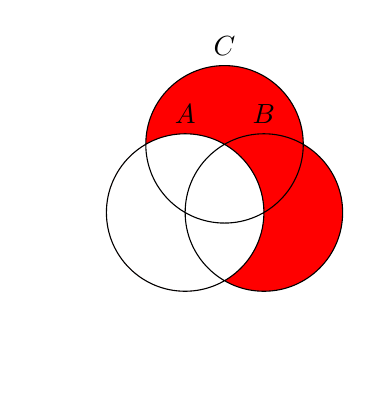
\begin{tikzpicture}[fill=red]
        % left hand
        \scope
        \clip (-2,-2) rectangle (2,2)
        (0,0) circle (1);
        \fill (0,0) circle (1);
        \endscope
        % right hand
        \scope
        \clip (-2,-2) rectangle (2,2)
        (0,0) circle (1);
        \fill (1,0) circle (1);
        \endscope
        \scope
        \clip (-2,-2) rectangle (2,2)
        (0,0) circle (1);
        \fill (0.5,0.866) circle (1);
        \endscope
        % outline
        \draw (0,0) circle (1) (0,1)  node [text=black,above] {$A$}
        (1,0) circle (1) (1,1)  node [text=black,above] {$B$}
        (0.5,0.866) circle (1) (0.5,1.866)  node [text=black,above] {$C$};
    \end{tikzpicture}
\end{align*}

% \subsubsection{Template for a venn diagrams:}

% \begin{align*}
%     \exp
% \end{align*}

\pagebreak

Here is a more complicated example involving 4 sets:

Refrenced from \url{https://www.overleaf.com/latex/examples/example-venn-diagram-with-isolated-areas-filled/xjptmqsjfdlc}

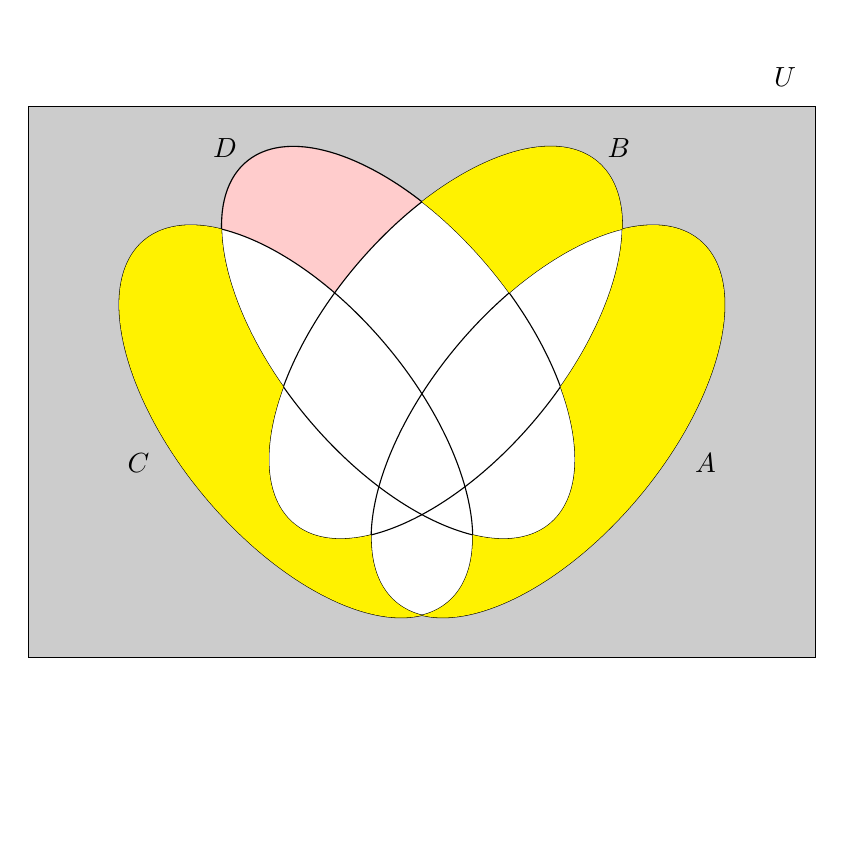
\begin{tikzpicture} \filldraw[fill=black, opacity=0.2] \bounding;

    \scope \fill[white] \fourthellip; \endscope \filldraw[fill=red,
        opacity=0.2] \fourthellip;

    %single colors
    \scope \fill[white] \secondellip; \fill[white] \thirdellip; \fill[white]
    \firstellip; \endscope

    \draw \firstellip node [label={[xshift=2.0cm, yshift=-0.9cm]$A$}] {};
    \draw \secondellip node [label={[xshift=2.2cm, yshift=2.1cm]$B$}] {};
    \draw \thirdellip node [label={[xshift=-2.0cm, yshift=-0.9cm]$C$}] {};
    \draw \fourthellip node [label={[xshift=-2.2cm, yshift=2.1cm]$D$}] {};
    \draw \bounding node [label=above left:$U$] {};

    \begin{scope}
        \begin{scope}[even odd rule]% first ellipse corner
            \clip \secondellip (-5,-5) rectangle (5,5);
            \clip \thirdellip (-5,-5) rectangle (5,5);
            \clip \fourthellip (-5,-5) rectangle (5,5);
            \fill[yellow] \firstellip;
        \end{scope}
    \end{scope}

    \begin{scope}
        \begin{scope}[even odd rule]% second ellipse corner
            \clip \firstellip (-5,-5) rectangle (5,5);
            \clip \thirdellip (-5,-5) rectangle (5,5);
            \clip \fourthellip (-5,-5) rectangle (5,5);
            \fill[yellow] \secondellip;
        \end{scope}
    \end{scope}

    \begin{scope}
        \begin{scope}[even odd rule]% third ellipse corner
            \clip \secondellip (-5,-5) rectangle (5,5);
            \clip \firstellip (-5,-5) rectangle (5,5);
            \clip \fourthellip (-5,-5) rectangle (5,5);
            \fill[yellow] \thirdellip;
        \end{scope}
    \end{scope}

\end{tikzpicture}

This covers the basics of set notation and operations.

\pagebreak

\subsection{Power sets}

The power set of a set is the set of all subsets of that set.

The power set of a set A is denoted in various ways, including $2^A$, $\mathcal{P}(A)$, $\mathbb{P}(A)$, or $\wp(A)$.

\begin{align*}
    \text{Let the set } A                 & = \{1, 2, 3\}                                                                   \\
    \wp(A)                                & = \{\emptyset, \{1\}, \{2\}, \{3\}, \{1, 2\}, \{1, 3\}, \{2, 3\}, \{1, 2, 3\}\} \\
    \text{More generally: } \mathbb{P}(A) & = \{B | B \subseteq A\}
\end{align*}

\subsection{Proofs}

\subsubsection{Proof by property}

Proposition (example from lecutre notes): For any sets A, B, and C:

\begin{align*}
    A\setminus (B\cup C) = (A\setminus B)\cap (A\setminus C)
\end{align*}

Recapping some of the basic properties of sets, using sets S and T, and element x:

\begin{align*}
     & \text{Property 1: } & S \subseteq T \text{ and } T \subseteq S  & \iff S = T               \\
     & \text{Property 2: } & (\text{For any x} \in S \implies x \in T) & \iff S \subseteq T       \\
     & \text{Property 3: } & x \in S \text{ and } x \in T              & \iff x \in S \cap T      \\
     & \text{Property 4: } & x \in S \text{ or } x \in T               & \iff x \in S \cup T      \\
     & \text{Property 5: } & x \in S \text{ and } x \notin T           & \iff x \in S \setminus T \\
     & \text{Property 6: } & x \notin S \text{ and } x \notin T        & \iff x \notin T \cup S   \\
\end{align*}

Using property 1, we can prove that two sets are equal by proving that each is a subset of the other.

\begin{align*}
     & \text{Let } x \in A\setminus (B\cup C)                                      \\
     & \iff x \in A \text{ and } x \notin B \cup C                                 \\
     & \iff x \in A \text{ and } x \notin B \text{ and } x \notin C                \\
     & \iff x \in A \setminus B \text{ and } x \in A \setminus C                   \\
     & \iff x \in (A \setminus B) \cap (A \setminus C)                             \\
     & \therefore A\setminus (B\cup C) \subseteq (A\setminus B)\cap (A\setminus C) \\
\end{align*}

Doing this for the other direction:

\begin{align*}
     & A\setminus (B\cup C)= (A\setminus B)\cap (A\setminus C)                           \\
     & \text{Let } x\in (A\setminus B)\cap (A\setminus C)                                \\
     & \iff x \in A\setminus B \text{ and } x \in A\setminus C                           \\
     & \iff x \in A \text{ and } x \notin B \text{ and } x \in A \text{ and } x \notin C \\
     & \iff x \in A \text{ and } x \notin B \cup C                                       \\
     & \iff x \in A \setminus (B \cup C)                                                 \\
     & \therefore (A\setminus B)\cap (A\setminus C) \subseteq A\setminus (B\cup C)
\end{align*}

\subsection{Von Neumann Ordinals}

The von Neumann ordinals are a way of representing the natural numbers using sets.


% let 0 = ∅
% let • 𝑛 + 1 = 𝑛 ∪ {𝑛}
let $0 = \emptyset$, $n + 1 = n \cup \{n\}$:

\begin{align*}
    0 & = \emptyset                                                                \\
    1 & = \{0\} = \{\emptyset\}                                                    \\
    2 & = \{0, 1\} = \{\emptyset, \{\emptyset\}\}                                  \\
    3 & = \{0, 1, 2\} = \{\emptyset, \{\emptyset\}, \{\emptyset, \{\emptyset\}\}\} \\
    n & = \{0, 1, 2, ..., n-1\} \text{ you get the idea}
\end{align*}

\section{Relations}

\subsection{Cartesian product and relations}

The cartesian product of two sets A and B is the set of all ordered pairs (x, y), where: $x \in A$ and $y \in B$.
The cartesian product of A and B is denoted as $A \times B$.

Example:

\begin{align*}
    Books               & = \{1984, \text{Concrete}, \text{Incerto}\}                                                                    \\
    Rating              & = \{\text{Good}, \text{Evil}, \text{Unimportant}\}                                                             \\
    Books \times Rating & = \{(1984, \text{Good}), (1984, \text{Evil}), (1984, \text{Unimportant})\}                                     \\
                        & \cup \{(\text{Concrete}, \text{Good}), (\text{Concrete}, \text{Evil}), (\text{Concrete}, \text{Unimportant})\} \\
                        & \cup \{(\text{Incerto}, \text{Good}), (\text{Incerto}, \text{Evil}), (\text{Incerto}, \text{Unimportant})\}
\end{align*}

A relation R from A to B is a subset of the cartesian product of A and B. i.e. $R \subseteq A \times B$.
Taking the example above, we can define a relation R from Books to Rating as:

\begin{align*}
    R = \{(1984, \text{Good}), (\text{Concrete}, \text{Evil}), (\text{Incerto}, \text{Unimportant})\}
\end{align*}

Note that R is a subset of the cartesian product of Books and Rating.

\subsection{Relation notation}

There are three main ways to denote a relation R from A to B:

\begin{itemize}
    \item Ordered pairs
    \item Table
    \item Mapping
\end{itemize}

Should you want to confuse yourself even further, the infix notation is a good option.

\begin{align*}
     & \text{Let the relation "likes" be defined as: } \mathbf{L} = \{(x, y) | x \text{ likes } y\} \\
     & \text{You can denote (x, y) as a subset of the likes by writing: x$\mathbf{L}$y}             \\
\end{align*}

\subsection{Representing relations}

Since winter is approaching, let's define a relation "likes" from people to clothing.

\begin{align*}
    \text{Let the set of people } P     & = \{\text{Jim}, \text{Bob}, \text{Alice}, \text{Eve}, \text{Mallory}\}     \\
    \text{Let the set of clothing } C   & = \{\text{Jacket}, \text{Scarf}, \text{Gloves}, \text{Hat}, \text{Socks}\} \\
    \text{Let the relation } \mathbf{L} & = \{(x, y) | x \text{ likes } y\}                                          \\
    \text{In table form:}                                                                                            \\
    \begin{tabular}{|l|l|l|l|l|l|l|}
        \hline
        P       & L      \\
        \hline
        Jim     & Scarf  \\
        \hline
        Bob     & Jacket \\
        \hline
        Alice   & Scarf  \\
        \hline
        Eve     & Gloves \\
        \hline
        Mallory & Hat    \\
        \hline
        Mallory & Socks  \\
        \hline
    \end{tabular}
\end{align*}

Since a table popped into your view, it is as good a time as any to introduce it's application in databases.

Given this example relation of students and their various attributes, we can represent it in a table.

\begin{align*}
    \text{Let the set of students } S   = \{\text{Jim}, \text{Bob}, \text{Alice}, \text{Eve}, \text{Mallory}\}                         \\
    \text{Let the set of attributes } A = \{\text{name}, \text{Age}, \text{Height}, \text{Weight}, text{Happiness}, \text{Net Worth}\} \\
    \text{Let the relation } \mathbf{R} = \{(x, y) | x \text{ has attribute } y\}                                                      \\
    \text{In table form:}                                                                                                              \\
    \begin{tabular}{|l|l|l|l|l|l|l|}
        \hline
        Name    & Age & Height & Weight & Happiness & Net Worth \\
        \hline
        Jim     & 20  & 180    & 80     & 0.5       & 0.1       \\
        \hline
        Bob     & 21  & 170    & 70     & 0.6       & 0.2       \\
        \hline
        Alice   & 19  & 160    & 60     & 0.7       & 0.3       \\
        \hline
        Eve     & 18  & 150    & 50     & 0.8       & 0.4       \\
        \hline
        Mallory & 17  & 140    & 40     & 0.9       & 0.5       \\
        \hline
    \end{tabular}
\end{align*}

We can extract information by getting a subset of relations.

For example: $(\text{Jim}, \text{180}) \in \text{Height}$

\subsection{Domain and range}

The domain of a relation is the set of all first elements of the ordered pairs in the relation.

\begin{align*}
    Dom(\mathbf{L}) & = \{x \in A \mid \exists x \in A : (x, y) \in \mathbf{L}\}
\end{align*}

The range of a relation is the set of all second elements of the ordered pairs in the relation.

\begin{align*}
    Ran(\mathbf{L}) & = \{y \in B \mid \exists y \in B : (x, y) \in \mathbf{L}\}
\end{align*}

\subsection{Relational composition}

The relational composition of two relations $\mathbf{R}$ and $\mathbf{S}$ is the relation $\mathbf{R} \circ \mathbf{S}$ (or $\mathbf{R};\mathbf{S}$, used to avoid confusion with function composition) defined as:

\begin{align*}
    \mathbf{R} ; \mathbf{S} & = \{(x, z) \mid \exists y \in B : (x, y) \in \mathbf{R} \text{ and } (y, z) \in \mathbf{S}\} \\
    \text{EXAMPLE:}                                                                                                        \\
    \mathbf{R}              & = \{(1, 2), (2, 3), (3, 4)\}                                                                 \\
    \mathbf{S}              & = \{(2, 3), (3, 4), (4, 5)\}                                                                 \\
    \mathbf{R} ; \mathbf{S} & = \{(1, 3), (2, 4), (3, 5)\}
\end{align*}

\subsection{Closures and equivalence classes}

\subsubsection{Property of relations}

A relation $\mathbf{R}$ is reflexive if $\forall x \in A : (x, x) \in \mathbf{R}$.

A relation $\mathbf{R}$ is symmetric if $\forall x, y \in A : (x, y) \in \mathbf{R} \implies (y, x) \in \mathbf{R}$.

A relation $\mathbf{R}$ is transitive if $\forall x, y, z \in A : (x, y) \in \mathbf{R} \text{ and } (y, z) \in \mathbf{R} \implies (x, z) \in \mathbf{R}$.



\subsubsection{Closures}

The closure of a relation $\mathbf{R}$ is the smallest relation containing $\mathbf{R}$ that is transitive.

Example of constructing a reflexive closure:

\begin{align*}
    \text{Let the relation } \mathbf{R}         & = \{(1, 2), (2, 3), (3, 4)\}                                 \\
    \text{The reflexive closure of } \mathbf{R} & = \{(1, 1), (1, 2), (2, 3), (3, 4), (2, 2), (3, 3), (4, 4)\}
\end{align*}

Example of constructing a symmetric closure:

\begin{align*}
    \text{Let the relation } \mathbf{R}         & = \{(1, 2), (2, 3), (3, 4)\}                         \\
    \text{The symmetric closure of } \mathbf{R} & = \{(1, 2), (2, 3), (3, 4), (2, 1), (3, 2), (4, 3)\}
\end{align*}

Example of constructing a transitive closure:

\begin{align*}
    \text{Let the relation } \mathbf{R}          & = \{(1, 2), (2, 3), (3, 4)\}                         \\
    \text{The transitive closure of } \mathbf{R} & = \{(1, 2), (2, 3), (3, 4), (1, 3), (2, 4), (1, 4)\}
\end{align*}


\subsubsection{Equivalence classes}

let $\rho \subseteq A \times A$ be an equivalence relation on A, given $A \neq \emptyset$, $a \in A$ be an arbitrary element of A.

NOTE: MUST CONSTRUCT EQUIVALENCE RELATION BEFORE CONSTRUCTING EQUIVALENCE CLASSES.

\begin{align*}
    [a]_{\rho} & = \{x \in A \mid (a, x) \in \rho\}
\end{align*}

\subsubsection{More properties of relations}

\begin{itemize}
    \item A relation $\mathbf{R}$ is antisymmetric if $\forall x, y \in A : (x, y) \in \mathbf{R} \text{ and } (y, x) \in \mathbf{R} \implies x = y$.
    \item A relation $\mathbf{R}$ is a partial order if it is reflexive, antisymmetric, and transitive.
    \item A connex relation is a relation $\mathbf{R}$ such that $\forall x, y \in A : (x, y) \in \mathbf{R} \text{ or } (y, x) \in \mathbf{R}$.
    \item Total order means that a relation is a partial order and a connex relation.
\end{itemize}
\section{Functions}

\subsection{Definition}

What is a function in the context of discrete mathematics?

A function is a relation $\mathbf{f}$ from A to B such that every element in A is mapped to exactly one element in B, i.e.:

$\forall x \in A . \forall y, z \in B : ((x, y) \in {f} \land (x, z) \in {f} \implies y = z)$.

\subsection{Notation}

A function $\mathbf{f}$ from A to B is denoted as $\mathbf{f} : A \rightarrow B$.

\subsection{Injective, surjective, bijective}

\begin{itemize}
    \item A function $\mathbf{f} : A \rightarrow B$ is injective if $\forall x, y \in A : \mathbf{f}(x) = \mathbf{f}(y) \implies x = y$.
    \item A function $\mathbf{f} : A \rightarrow B$ is surjective if $\forall y \in B : \exists x \in A : \mathbf{f}(x) = y$.
    \item A function $\mathbf{f} : A \rightarrow B$ is bijective if it is both injective and surjective.
\end{itemize}

\subsection{Composition}

The composition of two functions $\mathbf{f} : A \rightarrow B$ and $\mathbf{g} : B \rightarrow C$ is the function $\mathbf{g} \circ \mathbf{f} : A \rightarrow C$ defined as:

\begin{align*}
    \mathbf{g} \circ \mathbf{f} & = \{(x, z) \mid \exists y \in B : (x, y) \in \mathbf{f} \text{ and } (y, z) \in \mathbf{g}\}
\end{align*}

\subsection{Inverse}

The inverse of a function $\mathbf{f} : A \rightarrow B$ is the function $\mathbf{f}^{-1} : B \rightarrow A$ defined as:

\begin{align*}
    \mathbf{f}^{-1} & = \{(y, x) \mid (x, y) \in \mathbf{f}\}
\end{align*}

\section{Language and regular expressions}

\subsection{Alphabet}

We specify an Alphabet using the symbol $\Sigma$.

Examples:

\begin{align*}
    \Sigma_1 & = \{a, b, c, d, e, f\}                                                                                             \\
    \Sigma_2 & = \{0, 1, 2, 3, 4, 5, 6, 7, 8, 9\}                                                                                 \\
    \Sigma_3 & = \{S \mid S \subseteq \Sigma_1\}                     & (\text{The power set of } \Sigma_1, \#\Sigma_3 = 2^6 = 64) \\
    \Sigma_4 & = \{(x, y) \mid x \in \Sigma_1 \land y \in \Sigma_2\} & \text{Ordered pairs of characters work as well}
\end{align*}

An alphabet must be a set that contain finite elements,
hence sets like $\mathbb{N} = \{1,2,3,4,5,6,7,8,9,...\}$ cannot be the alphabet of a language.

\subsection{Strings}

A string is a finite sequence of characters from an alphabet.

A string of length n is denoted as the n-tuple $w = a_1a_2a_3...a_n$, written without punctuation.

The set of all finite strings are denoted as $\Sigma^*$, and we can say that string s is in $\Sigma^*$ if $s \in \Sigma^*$.

\subsubsection{Empty string}

Might be jarring to you, Jim, but you have the option to denote an empty string as $\epsilon$. Will be useful later on.

\subsubsection{String Operations}

\begin{itemize}
    \item Concatenation: $w_1w_2$ is the concatenation of strings $w_1$ and $w_2$.
    \item Length: $|w|$ is the length of string w. The length of concatenated strings are simply the sum of the lengths of the individual strings.
\end{itemize}

\subsection{Language}

A language is a set of strings.

\subsection{Regular expressions}

A regular expression is a string that denotes a language. Here are the rules:

\begin{itemize}
    \item lwt$\Sigma$ be an alphabet.
    \item $a$ denotes the language $\{a\}$, where $a \in \Sigma$, which is on its own a regular expression.
    \item $\epsilon$ and $\emptyset$ denote the languages $\{\epsilon\}$ and $\emptyset$, which are also regular expressions.
    \item Given r and s as regular expressions, the following are also regular expressions:
          \begin{itemize}
              \item $rs$, $r|s$, $r^*$
          \end{itemize}
\end{itemize}

\subsubsection{Examples}

The following are rules for matching strings to RegEx, let s be a string and r be a regular expression:

\begin{itemize}
    \item $s$ matches $a$ when $s = a$
    \item $\epsilon$ matches $\epsilon$ when $s = \epsilon$
    \item $\emptyset$ matches nothing.
    \item $r|s$ matches $r$ or $s$.
    \item $rs$ matches $r$ followed by $s$.
    \item $r^*$ matches if $s = \epsilon$ or $s = s_1s_2...s_n$, where $s_i$ matches $r$ for all $i$.
\end{itemize}

\subsubsection{Regular languages}

A language is regular if it is denoted by a regular expression.

\begin{align*}
    \text{For alphabet $\Sigma$ and regular expressions r:} \\
    L(r) = \{s \in \Sigma^* \mid s \textbf{ matches } r\}
\end{align*}

\section{Finite automata}

\subsection{Deterministic finite automata}

\begin{align*}
    \text{States: } Q                 & = \{q_0, q_1, q_2, q_3\}        \\
    \text{Symbol: } \Sigma            & = \{0, 1\}                      \\
    \text{Transition Function} \delta & : Q \times \Sigma \rightarrow Q \\
    \text{Start: }                    & = q_0 \in Q                     \\
    \text{Accepting: }                & = \{q_2, q_3\} \subseteq Q      \\
    \text{DFA$(^\epsilon)$: } M       & = (Q, \Sigma, \delta, q_0, \{q_2, q_3\})
\end{align*}


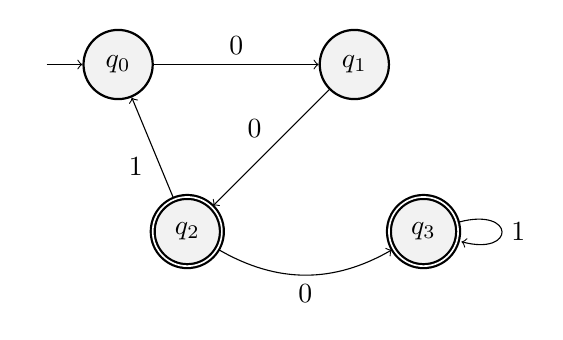
\begin{tikzpicture}
    \node[state, initial] (q0) {$q_0$};
    \node[state, right of = q0] (q1) {$q_1$};
    \node[state, accepting, below left of = q1] (q2) {$q_2$};
    \node[state, accepting, right of = q2] (q3) {$q_3$};
    \draw (q0) edge[above] node{0} (q1)
    (q1) edge[above left] node{0} (q2)
    (q2) edge[below left] node{1} (q0)
    (q2) edge[bend right, below] node{0} (q3)
    (q3) edge[loop right] node{1} (q3);
\end{tikzpicture}

\subsubsection{Criteria for a DFA}

\begin{itemize}
    \item DFAs have exactly one start state.
    \item May have one or more accepting states.
    \item For each state, there must be at most one outgoing transition $\textbf{for each symbol in the alphabet.}$
\end{itemize}

\subsubsection{Language definition with DFAs}

For automaton $M$, the language $L(M)$ consists of all strings $s$ over its alphabet of input symbols statisfying:

\begin{align}
    & q_0 \xrightarrow{\text{s}} * q \\
    & s = q_0,q_1,q_2,...,q_n \text{ for the states: } q_0, q_1, q_2, ..., q_n
\end{align}

If (1) is the case, $s$ is accepted by $M$.
More formally:

\begin{align*}
    L(M) = \{u \mid u \textbf{ is accepted by } M\}
\end{align*}

\subsection{Non-deterministic finite automata}

\subsubsection{What is the difference?}

\begin{itemize}
    \item NDFAs can have multiple outgoing transitions for a given symbol.
    \item NDFAs can have $\epsilon$-transitions, which are transitions that can be taken without consuming an input symbol.
    \item NDFAs can have multiple start states.
    \item NDFAs can have no accepting states.
    \item NDFAs can have multiple accepting states.
\end{itemize}
\subsection{Examples}

Referenced from \url{https://www3.nd.edu/~kogge/courses/cse30151-fa17/Public/other/tikz_tutorial.pdf}.

\subsubsection{DFA 1}

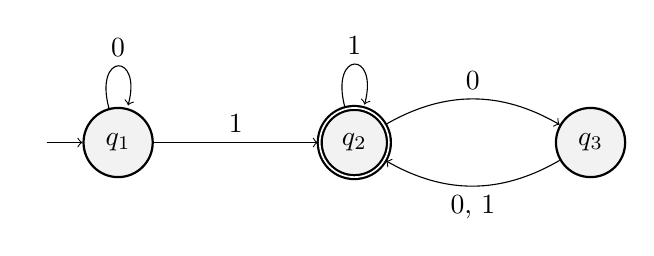
\begin{tikzpicture}
    \node[state, initial] (q1) {$q_1$};
    \node[state, accepting, right of=q1] (q2) {$q_2$};
    \node[state, right of=q2] (q3) {$q_3$};
    \draw (q1) edge[loop above] node{0} (q1)
    (q1) edge[above] node{1} (q2)
    (q2) edge[loop above] node{1} (q2)
    (q2) edge[bend left, above] node{0} (q3)
    (q3) edge[bend left, below] node{0, 1} (q2);
\end{tikzpicture}

\subsubsection{NFA 1}

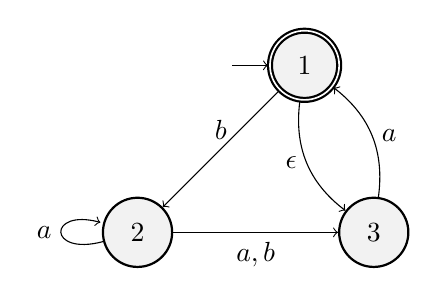
\begin{tikzpicture}
    \node[state, initial, accepting] (1) {$1$};
    \node[state, below left of=1] (2) {$2$};
    \node[state, right of=2] (3) {$3$};
    \draw (1) edge[above] node{$b$} (2)
    (1) edge[below, bend right, left=0.3] node{$\epsilon$} (3)
    (2) edge[loop left] node{$a$} (2)
    (2) edge[below] node{$a, b$} (3)
    (3) edge[above, bend right, right=0.3] node{$a$} (1);
\end{tikzpicture}

\subsubsection{DFA 2}

\begin{figure}
\centering
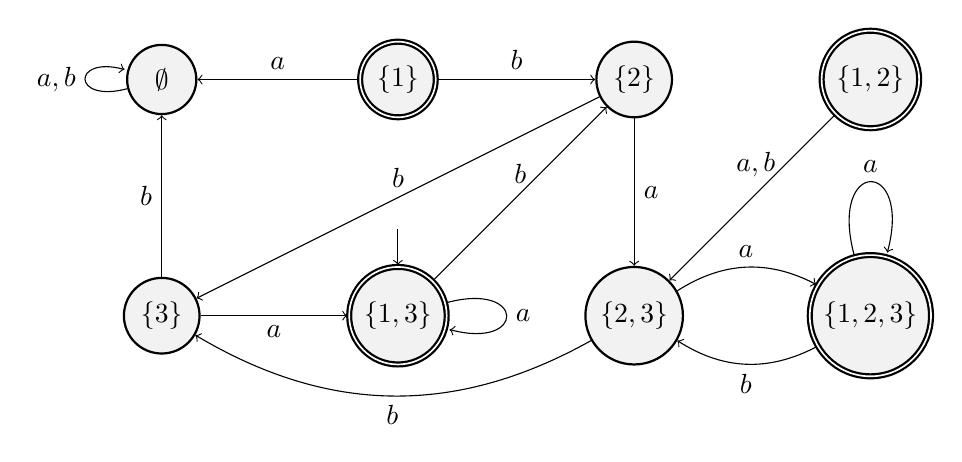
\begin{tikzpicture}
    \node[state] (phi) {$\emptyset$};
    \node[state, accepting, right of=phi] (1) {$\{1\}$};
    \node[state, right of=1] (2) {$\{2\}$};
    \node[state, accepting, right of=2] (12) {$\{1, 2\}$};
    \node[state, below of=phi] (3) {$\{3\}$};
    \node[state, initial, initial where=above, accepting, right of=3] (13) {$\{1, 3\}$};
    \node[state, right of=13] (23) {$\{2, 3\}$};
    \node[state, accepting, right of=23] (123) {$\{1, 2, 3\}$};
    5
    \draw (phi) edge[loop left] node{$a, b$} (phi)
    (1) edge[above] node{$a$} (phi)
    (1) edge[above] node{$b$} (2)
    (2) edge[right] node{$a$} (23)
    (2) edge[above] node{$b$} (3)
    (12) edge[above, pos=.3, left=2pt] node{$a, b$} (23)
    (3) edge[left] node{$b$} (phi)
    (3) edge[below] node{$a$} (13)
    (13) edge[loop right] node{$a$} (13)
    (13) edge[above] node{$b$} (2)
    (23) edge[bend left, above] node{$a$} (123)
    (23) edge[bend left, below] node{$b$} (3)
    (123) edge[loop above] node{$a$} (123)
    (123) edge[bend left, below] node{$b$} (23);
\end{tikzpicture}
\caption{DFA} \label{fig:DFA}
\end{figure}


\section{logic}

\section{Graphs and trees}

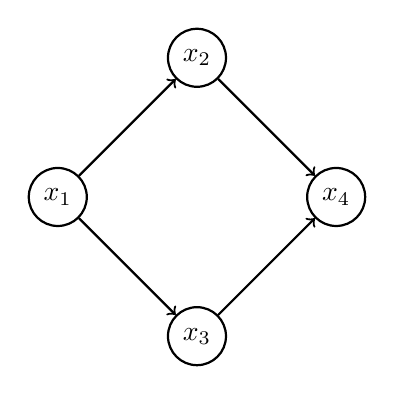
\begin{tikzpicture}[node distance={25mm}, thick, main/.style = {draw, circle}] 
    \node[main] (1) {$x_1$}; 
    \node[main] (2) [above right of=1] {$x_2$}; 
    \node[main] (3) [below right of=1] {$x_3$}; 
    \node[main] (4) [above right of=3] {$x_4$}; 
    \draw[->] (1) -- (2); 
    \draw[->] (1) -- (3); 
    \draw (2) -- (4); 
    \draw (3) -- (4); 
\end{tikzpicture}

Ayyy lmao.

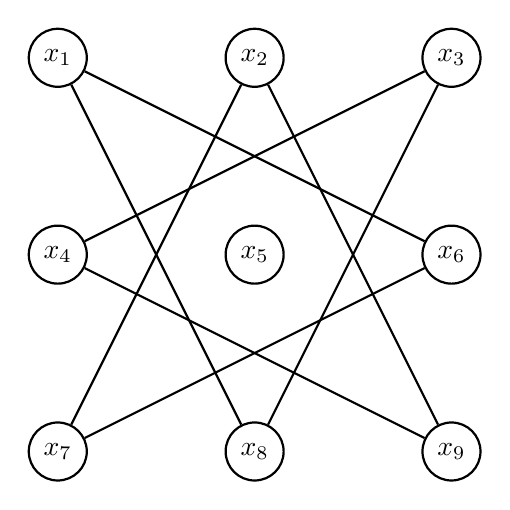
\begin{tikzpicture}[node distance={25mm}, thick, main/.style = {draw, circle}] 
    \node[main] (1) {$x_1$}; 
    \node[main] (2) [right of=1] {$x_2$}; 
    \node[main] (3) [right of=2] {$x_3$}; 
    \node[main] (4) [below of=1] {$x_4$};
    \node[main] (5) [right of=4] {$x_5$};
    \node[main] (6) [right of=5] {$x_6$};
    \node[main] (7) [below of=4] {$x_7$};
    \node[main] (8) [right of=7] {$x_8$};
    \node[main] (9) [right of=8] {$x_9$};
    \draw [-] (1) -- (6); 
    \draw [-] (1) -- (8);
    \draw [-] (3) -- (4);
    \draw [-] (3) -- (8);
    \draw [-] (4) -- (9);
    \draw [-] (9) -- (2);
    \draw [-] (2) -- (7);
    \draw [-] (7) -- (6);
\end{tikzpicture}

Now onto the 3 $\times$ 4 example.

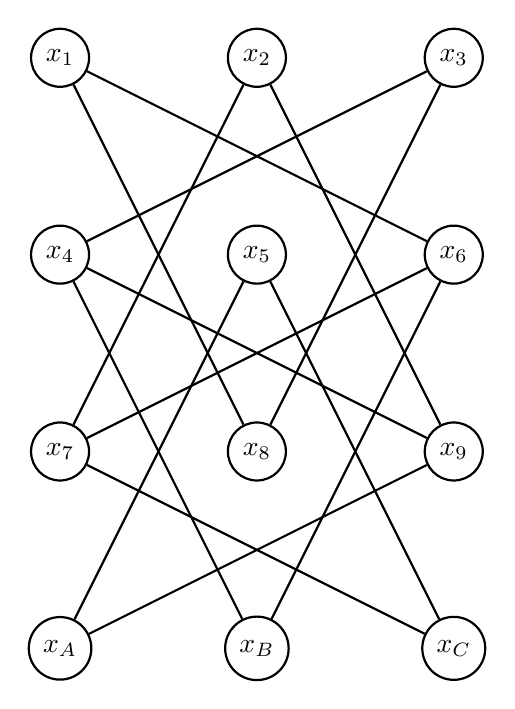
\begin{tikzpicture}[node distance={25mm}, thick, main/.style = {draw, circle}] 
    \node[main] (1) {$x_1$}; 
    \node[main] (2) [right of=1] {$x_2$}; 
    \node[main] (3) [right of=2] {$x_3$}; 
    \node[main] (4) [below of=1] {$x_4$};
    \node[main] (5) [right of=4] {$x_5$};
    \node[main] (6) [right of=5] {$x_6$};
    \node[main] (7) [below of=4] {$x_7$};
    \node[main] (8) [right of=7] {$x_8$};
    \node[main] (9) [right of=8] {$x_9$};
    \node[main] (10) [below of=7] {$x_A$};
    \node[main] (11) [right of=10] {$x_B$};
    \node[main] (12) [right of=11] {$x_C$}; 

    \draw [-] (1) -- (6); 
    \draw [-] (1) -- (8);
    \draw [-] (3) -- (4);
    \draw [-] (3) -- (8);
    \draw [-] (4) -- (9);
    \draw [-] (9) -- (2);
    \draw [-] (2) -- (7);
    \draw [-] (7) -- (6);
    \draw [-] (4) -- (11);
    \draw [-] (11) -- (6);
    \draw [-] (12) -- (5);
    \draw [-] (12) -- (7);
    \draw [-] (5) -- (10);
    \draw [-] (10) -- (9);
\end{tikzpicture}

\pagebreak

\section{Proofs}

\subsection{introduction}


Proofs are hard to write, but easy to read.
Proof that the sum of an even number and odd number is odd:

\begin{align*}
    \text{Let } x & = 2k \text{ where } k \in \mathbb{Z} \\
    \text{Let } y & = 2k + 1 \text{ where } k \in \mathbb{Z} \\
    x + y & = 2k + 2k + 1 \\
    & = 4k + 1 \\
    & = 2(2k) + 1 \\
    & = 2k' \text{ where } k' \in \mathbb{Z} \\
    & \therefore x + y \text{ is odd}
\end{align*}



\end{document}
